\chapter{Problemes del SDK connectat a producció}

    \paragraph{}
    Aquesta secció neix en el nostre projecte, en gran part, fruit de la curiositat. No representava un objectiu del projecte, explorar les dades de producció, accessibles a través del SDK o l'API, però el fet d'aconseguir aquest accés i disposar d'alguns dies, en els quals podíem fer un esforç i explorar-lo, ens ha animat a jugar una mica amb l'entorn de producció.

    Mitjançant la utilització de les funcionalitats implementades en la prova pilot, hem pogut observar dos problemes en la interacció del SDK amb l'API de FamilySearch. A continuació, exposem aquests dos problemes, de forma més detallada.

    \section{Paràmetres de cerca no funcionals}

\subsection{Introducció i demostració}

\paragraph{}
Com ja havíem anunciat en la funcionalitat cerca de persones a l'arbre familiar, exposada en l'apartat~\ref{sec:searchTree}, sembla que els paràmetres de cerca referents a les localitzacions i dates de naixement, casament i defunció, pels relatius de la persona cercada, de forma contrària als paràmetres disponibles especificats en les documentacions de l'API de FamilySearch i del SDK, no funcionen.

Introduíem aquest fet ja en la funcionalitat, perquè aquest comportament era detectable en l'entorn `sandbox', però volíem comprovar-ho també a producció. Per fer-ho, utilitzarem el següent conjunt de persones de l'arbre familiar:

\begin{itemize}
    \item Principal persona cercada
    \begin{itemize}
        \item Nom: Maria Eliza
        \item Cognom: Williams
        \item Naixement: 20 September 1857 / La Moille, Bureau, Illinois, United States
        \item Defunció: 9 July 1935 / Los Angeles, California, United States
    \end{itemize}
    \item Parella de la persona cercada
    \begin{itemize}
        \item Nom: Albert
        \item Cognom: Porter
        \item Naixement: 1844
        \item Defunció: 1925
    \end{itemize}
    \item Pare de la persona cercada
    \begin{itemize}
        \item Nom: Solomon
        \item Cognom: Williams
        \item Naixement: 1809
        \item Defunció: 1887
    \end{itemize}
    \item Mare de la persona cercada
    \begin{itemize}
        \item Nom: Frances
        \item Cognom: Prime
        \item Naixement: 1828
        \item Defunció: NA
    \end{itemize}
\end{itemize}

Per demostrar el no funcionament d'alguns dels paràmetres, procedirem a rea\-lit\-zar diferents cerques i a observar-ne els resultats.

En primer lloc, si utilitzem els paràmetres \emph{nom} i \emph{cognom} de la principal persona cercada, el SDK retorna un total de 52 persones (figura~\ref{fig:maria1}).

\begin{figure}[h]
    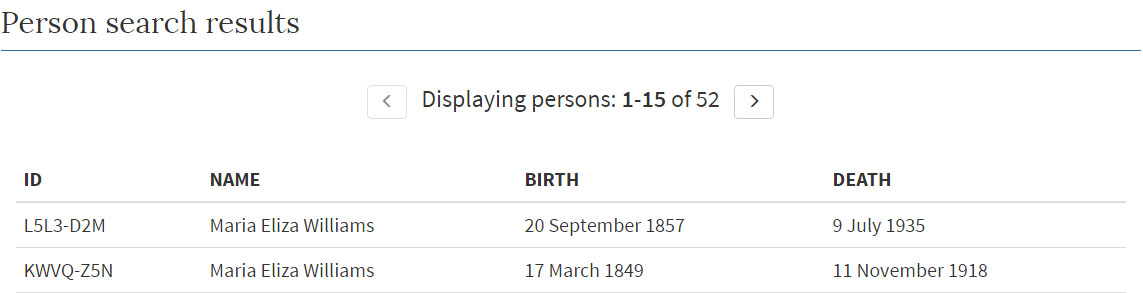
\includegraphics[width=\linewidth]{11.5/01_maria1}
    \centering
    \caption{Cerca amb nom i cognom de la principal persona cercada}\label{fig:maria1}
\end{figure}

En segon lloc, si concretem la informació sobre la principal persona cercada, incloent-hi els paràmetres data i lloc de naixement i data i lloc de defunció, passem a obtenir només la persona que desitgem de l'arbre familiar (figura~\ref{fig:maria2}).

\begin{figure}[h]
    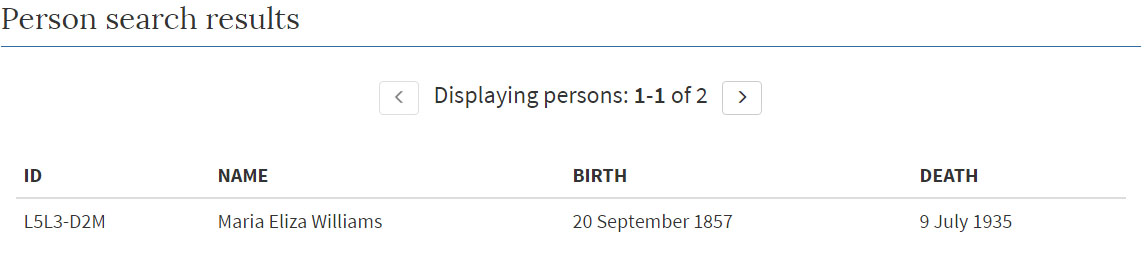
\includegraphics[width=\linewidth]{11.5/02_maria2}
    \centering
    \caption{Cerca detallada o cerca amb nom i cognom dels relatius}\label{fig:maria2}
\end{figure}

De la mateixa forma, per confirmar que la cerca mitjançant els noms i cognoms dels familiars més propers funciona, realitzem una cerca utilitzant només el \emph{nom} i \emph{cognom} de la principal persona cercada, la parella, el pare i la mare. El resultat, de la mateixa forma que la cerca anterior, només una persona (figura~\ref{fig:maria2}).

Així doncs, es veu clar que els paràmetres \emph{nom} i \emph{cognom} dels relatius, sí que funcionen i és més, ens ajuden a reduir el nombre de resultats, de les 52 persones elegibles utilitzant només el \emph{nom} i \emph{cognom} de la persona cercada, a només 1 resultat.

No obstant això, tan  bon punt afegim qualsevol paràmetre, com per exemple, l'any de naixement del pare, la cerca produeix zero resultats (imatge~\ref{fig:maria3}). El mateix resultat és obtingut si s'utilitza qualsevol localització o any, relacionat amb els principals esdeveniments, dels relatius més propers de la persona cercada.

\begin{figure}[h]
    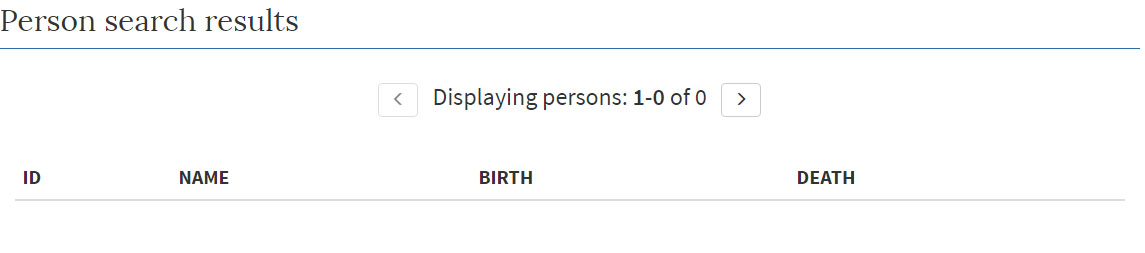
\includegraphics[width=\linewidth]{11.5/03_maria3}
    \centering
    \caption{Cerca amb el paràmetre any de neixement del pare}\label{fig:maria3}
\end{figure}


\subsection{Implicacions del problema}

\paragraph{}
Les implicacions d'aquest problema són bastant evidents. Simplement, aquests paràmetres de cerca no poden ser utilitzats.

Desconeixem el motiu pel qual aquests paràmetres es troben especificats en la documentació oficial com a utilitzables, però la realitat, és que ni la mateixa organit\-zació els utilitza en la seva funcionalitat de cerca a l'arbre genealògic. (figura~\ref{fig:searchofi}).

\begin{figure}[h]
    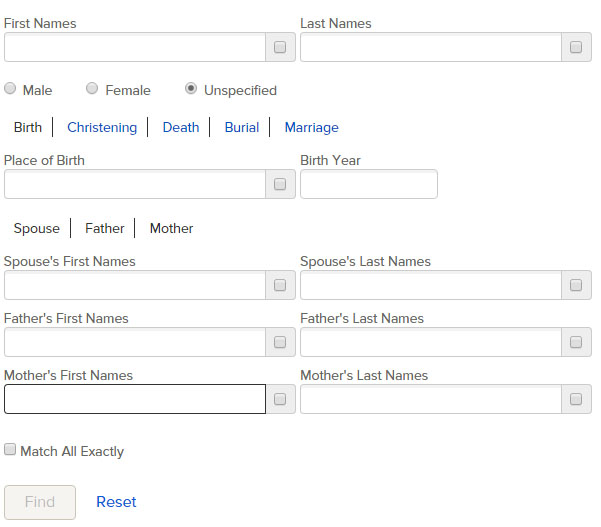
\includegraphics[scale=0.4]{11.5/04_oficialSearcher}
    \centering
    \caption{Formulari oficial de cerca a l'arbre familiar, de FamilySearch}\label{fig:searchofi}
\end{figure}

    \section{Cerca de persones per localitzacions: Incompleta}

\subsection{Introducció i demostració}

\paragraph{}
Aquest problema és detectat quan obtenim accés a producció i comencem a jugar amb la funcionalitat evolució d'esdeveniments, ja que en l'entorn de producció `sandbox', no era detectable.

La prova pilot d'aquesta funcionalitat, es basava en la cerca a l'arbre familiar, per només una localització sobre el lloc de naixement, casament o defunció.

Quan es comencen a realitzar proves en l'entorn de producció, el nombre de resultats retornats per cada any de l'interval d'onze anys, és definitivament més baix del que esperàvem. Per comprendre el que estava passant, vam realitzar una investigació a través de la funcionalitat de cerca, també implementada en la prova pilot.

En la primera cerca de prova, demanem a la funcionalitat cerca de persones, que retorni totes les persones nascudes als Estats Units. Sorprenentment, la cerca només retorna 168.117 resultats (figura~\ref{fig:searchStates}).

\begin{figure}[h]
    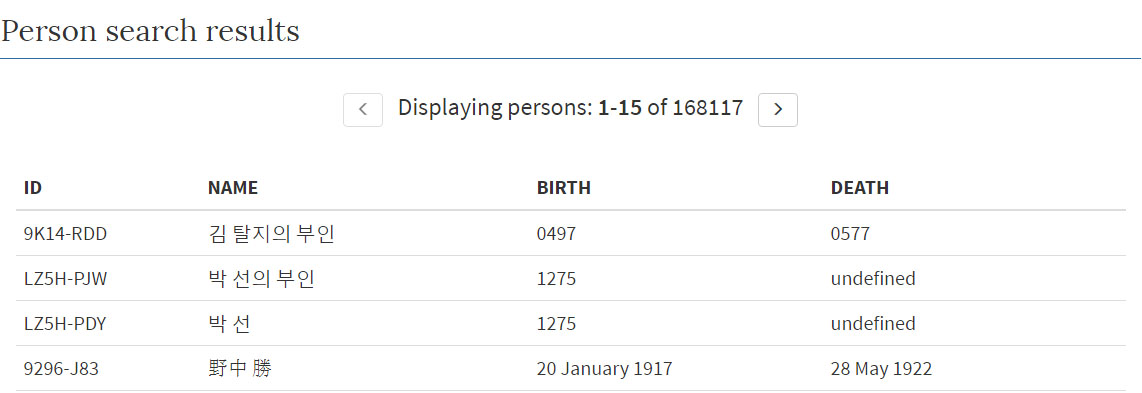
\includegraphics[width=\linewidth]{11.5/00_places}
    \centering
    \caption{Cerca per persones nascudes als Estats Units}\label{fig:searchStates}
\end{figure}

Aquest nombre és evidentment incorrecte, perquè si realitzem una cerca per aquelles persones que es diuen Tom i que a més a més, han nascut als Estats Units, la cerca retorna 2.909.316 persones (figura~\ref{fig:searchTom}). Aquest nombre, que ``en principi hauria de ser més petit'' que el retornat per la primera cerca, ens indica que alguna cosa no acaba de funcionar en la cerca del SDK.

\begin{figure}[h]
    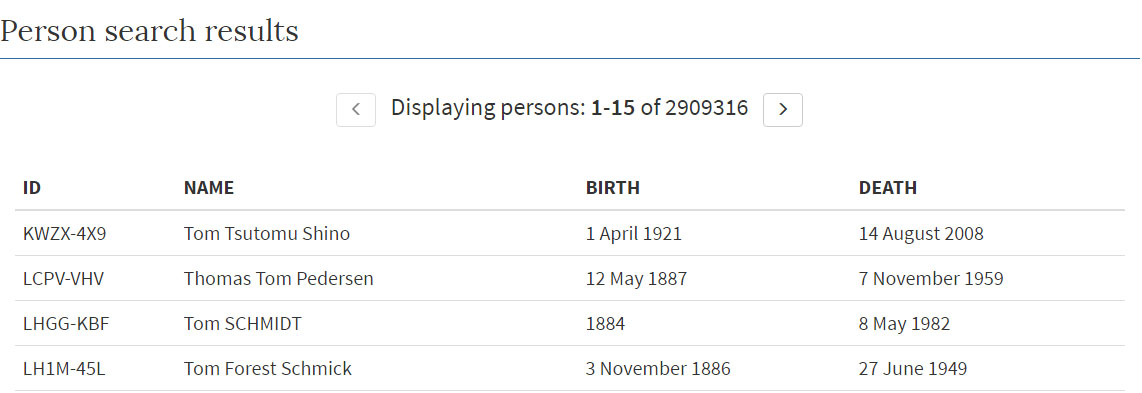
\includegraphics[width=\linewidth]{11.5/01_places}
    \centering
    \caption{Cerca per persones amb nom Tom i nascudes als Estats Units}\label{fig:searchTom}
\end{figure}

Així doncs, si ens fixem en els resultats retornats en la resposta de la primera cerca (figura~\ref{fig:searchStates}), podem observar com tots els resultats retornats semblen contenir caràcters no llatins. En altres paraules, el conjunt de persones retornades sembla estar format per Coreans, Japonesos, Xinesos, etcètera, etcètera.

Aquest fet ens fa sospitar que la funcionalitat de cerca és incapaç de retornar resultats correctes, si no s'especifica algun dels paràmetres nom i cognom, per la persona cercada o algun dels familiars més propers.

Aquesta hipòtesi es veu reforçada al realitzar més comprovacions. Al final, es pot concloure que el motiu pel qual la primera cerca retornava 165.952 persones, era perquè aquest és el col·lectiu de persones que complia la condició de cerca en què el nom o cognom, no estava format per caràcters llatins o estaven buits.


\subsection{Implicacions del problema}

\paragraph{}
El primer que caldria comprovar és si aquest problema també succeeix mitjançant la connexió directa amb l'API de FamilySearch. En cas de ser així, probablement aquest obstacle no seria superable de forma directa i implicaria que la cerca global de persones, a través de la introducció d'una localització de naixement, casament o defunció, no es troba suportada pel sistema.

Aquesta restricció també significa, que almenys, a través del SDK, la funcionalitat d'evolució d'esdeveniments que havíem plantejat en la prova pilot, no acabaria de funcionar i caldria trobar mètodes alternatius, per tal de poder produir gràfics basats en una quantitat de dades més elevada.

Per exemple, realitzar la cerca pels noms o cognoms més comuns del país introduït i agregar les dades o realitzar directament la cerca per una localització i cognom especificats per l'usuari, en comptés de només una localització.

El que està clar, és que és una restricció a tenir en compte de cara a la rea\-lit\-za\-ció de futurs projectes, si és que es confirma que aquest problema també existeix mitjançant la connexió directa a l'API.

De totes maneres, sempre existeixen alternatives que poden permetre afrontar les tasques de forma indirecta i aquest problema s'ha fet latent a l'organització Family\-Search, a través del grup per desenvolupadors, amb l'esperança de què pugui ser adreçat en un futur.

